\documentclass{article}
\usepackage[a4paper, paperwidth=25cm, paperheight=25.5cm, left=1.5cm, right=1.5cm, top=1cm, bottom=2cm]{geometry}
\usepackage{tikz,tcolorbox}
\usepackage{amsmath}
\usepackage[table,xcdraw]{xcolor}
\usepackage{listings}
\usepackage{array,multirow} % For customizing tables
\usepackage{booktabs} % For better horizontal lines
\usepackage{makecell}
\setlength{\parindent}{0pt}

\lstset{
    language=SQL,                    % Set language to SQL
    basicstyle=\ttfamily\small,      % Font size and family for code
    keywordstyle=\color{blue}\bfseries, % Color for SQL keywords
    commentstyle=\color{gray},       % Color for comments
    stringstyle=\color{red},         % Color for strings
    numbers=left,                    % Show line numbers on the left
    numberstyle=\tiny\color{gray},   % Line number font and color
    stepnumber=1,                    % Line number step
    breaklines=true,                 % Wrap long lines
    frame=single,                    % Add a frame around code
    tabsize=2,                       % Set tab size
    showstringspaces=false           % Hide spaces in strings
}


\newcommand{\partie}[1]{
  \section*{Partie #1}
  \vspace{-0.5cm}
  \noindent\rule{\textwidth}{0.5pt}%
}

\newcommand{\tit}[1]{
\begin{center}
    \Large{\textbf{{#1}}}
\end{center}
}

\definecolor{commentgray}{HTML}{676160}
\definecolor{messagegreen}{HTML}{17B867}
\definecolor{myblue}{HTML}{10C2C4}

\tcbuselibrary{skins, breakable, theorems}


\newtcolorbox{prettyBox}[2]{
  enhanced,
  colback=white!90!#2,   % Background color based on the second parameter (color)
  colframe=#2!60!black,  % Frame color based on the second parameter (color)
  coltitle=white,        % Title color (white)
  fonttitle=\bfseries\Large,
  title=#1,              % Title from the first parameter
  boxrule=1mm,
  arc=0.5mm,
  drop shadow=#2!35!gray, % Drop shadow color based on the second parameter (color)
}



\begin{document}
\tit{Devoir Maison N\(^{\boldsymbol{\circ}}\)\hspace{0.1cm}1}

\partie{0}
\section{Creation De La Base De Donne}

\textbf{\underline{Code}}
\lstinputlisting{Parties/Partie0/createDB.sql}

\vspace{1cm}
\textbf{\underline{Output}}
\vspace{1cm}
\begin{center}
    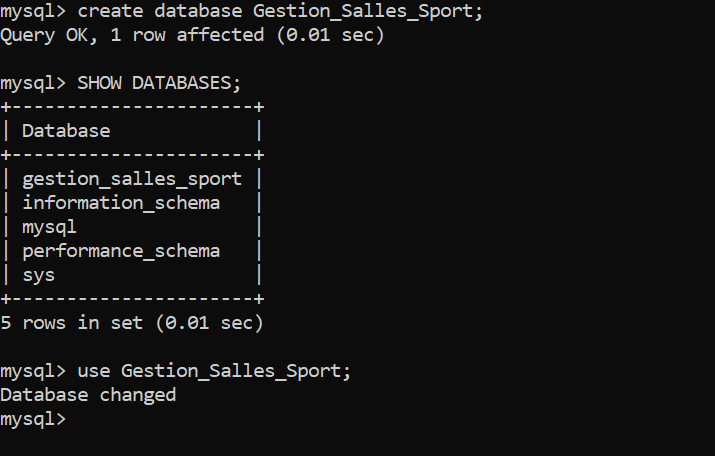
\includegraphics[height=0.5\textheight]{Parties/Partie0/Capture.PNG}
\end{center}



\newpage
\partie{1}
\section{Creation Des Tables}
\subsection{Sportifs}
\lstinputlisting{Parties/Partie1/CreateTables/createSportifs.sql}

\vspace{0.25cm}

\subsection{Sports}
\lstinputlisting{Parties/Partie1/CreateTables/createSports.sql}

\vspace{0.25cm}

\subsection{Gymnases}
\lstinputlisting{Parties/Partie1/CreateTables/createGymnases.sql}

\vspace{0.25cm}

\subsection{Arbitrer}
\lstinputlisting{Parties/Partie1/CreateTables/createArbitrer.sql}

\vspace{0.25cm}

\subsection{Entrainer}
\lstinputlisting{Parties/Partie1/CreateTables/createEntrainer.sql}

\vspace{0.25cm}

\subsection{Jouer}
\lstinputlisting{Parties/Partie1/CreateTables/createJouer.sql}

\vspace{0.25cm}

\subsection{Seances}
\lstinputlisting{Parties/Partie1/CreateTables/createSeance.sql}

\newpage

\textbf{\underline{Verification Des Table Crees}}
\vspace{1cm}
\begin{center}
    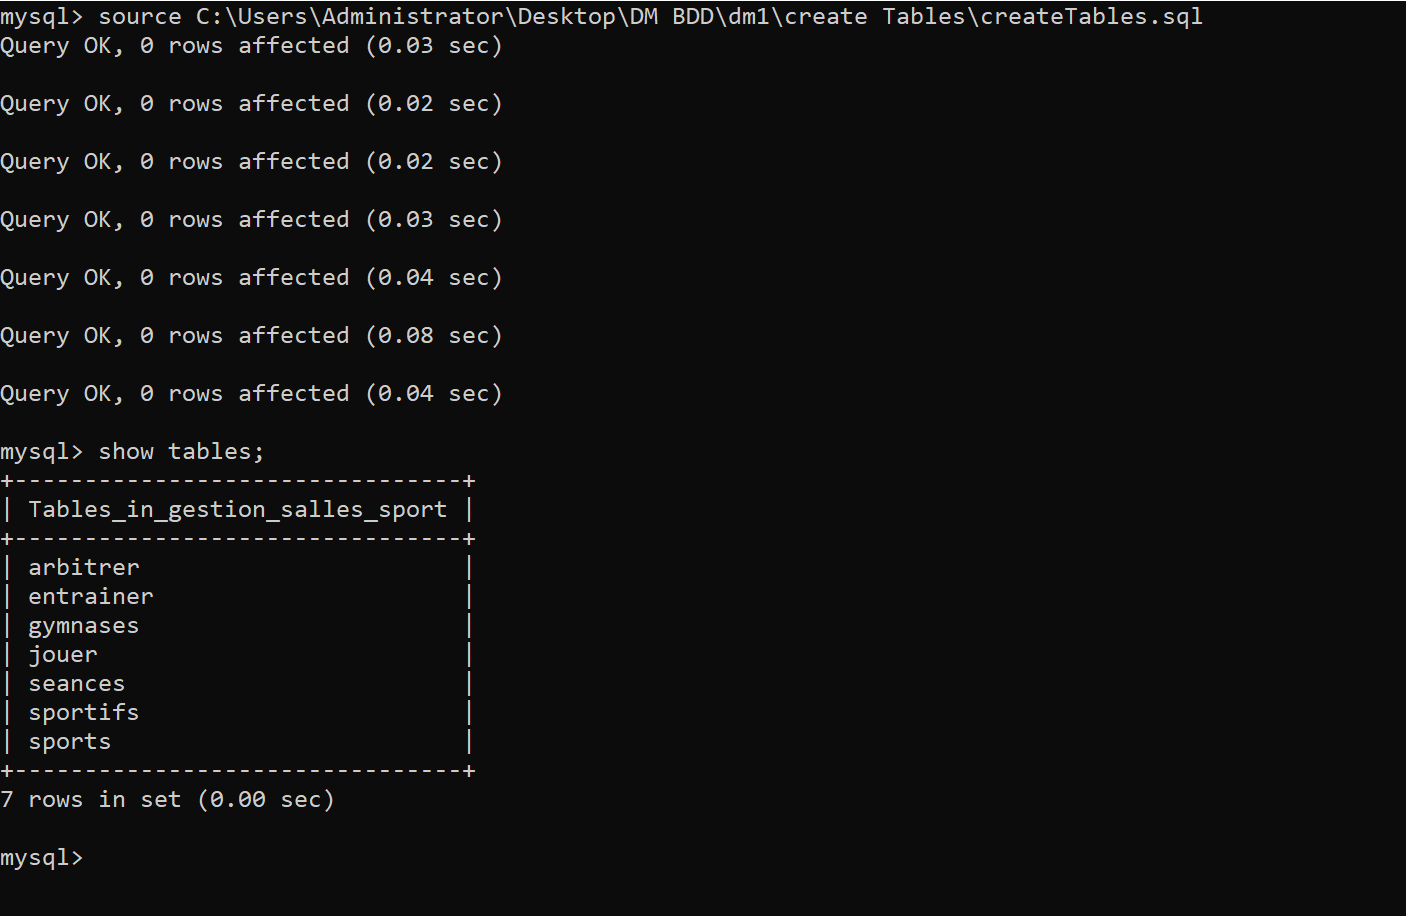
\includegraphics[height=0.6\textheight]{Parties/Partie1/CreateTables/showTables.PNG}
\end{center}

\newpage
\section{Ajouter L'attribut \texttt{DateCreation} A La Table \texttt{Gymnases}}
\lstinputlisting{Parties/Partie1/q2.sql}

\vspace{1cm}
\section{Ajouter La Contrainte \texttt{Not Null} Aux Attributs \texttt{SEXE} et \texttt{Age} De La Table \texttt{Sportifs}}
\lstinputlisting{Parties/Partie1/q3.sql}

\vspace{1cm}
\section{Modifier La Taille De L'Attribut \texttt{Prenom} De La Table \texttt{Sportifs}}
\lstinputlisting{Parties/Partie1/q4.sql}

\vspace{1cm}
\section{Suppression De L'attribut \texttt{DateCreation} A La Table \texttt{Gymnases}}
\lstinputlisting{Parties/Partie1/q5.sql}

\vspace{0.25cm}
\textbf{\underline{Output}}
\vspace{0.25cm}
\begin{center}
    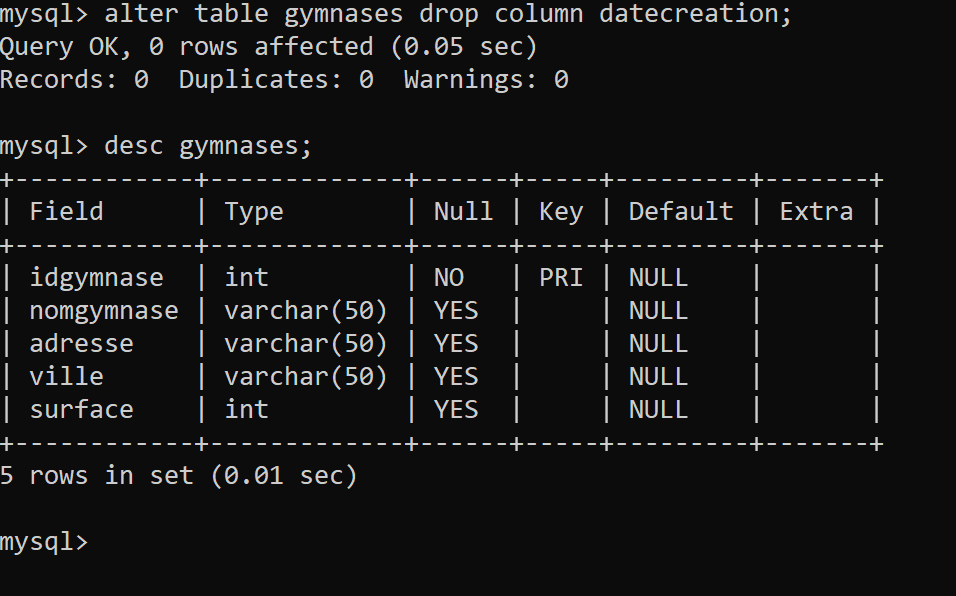
\includegraphics[height=0.36\textheight]{Parties/Partie1/drop.PNG}
\end{center}

\newpage

\section{Renommer L'attribut \texttt{ADRESSE} A La Table \texttt{Gymnases} Par \texttt{ADRESSEGYM}}
\lstinputlisting{Parties/Partie1/q6.sql}

\vspace{0.25cm}
\textbf{\underline{Output}}
\vspace{0.25cm}
\begin{center}
    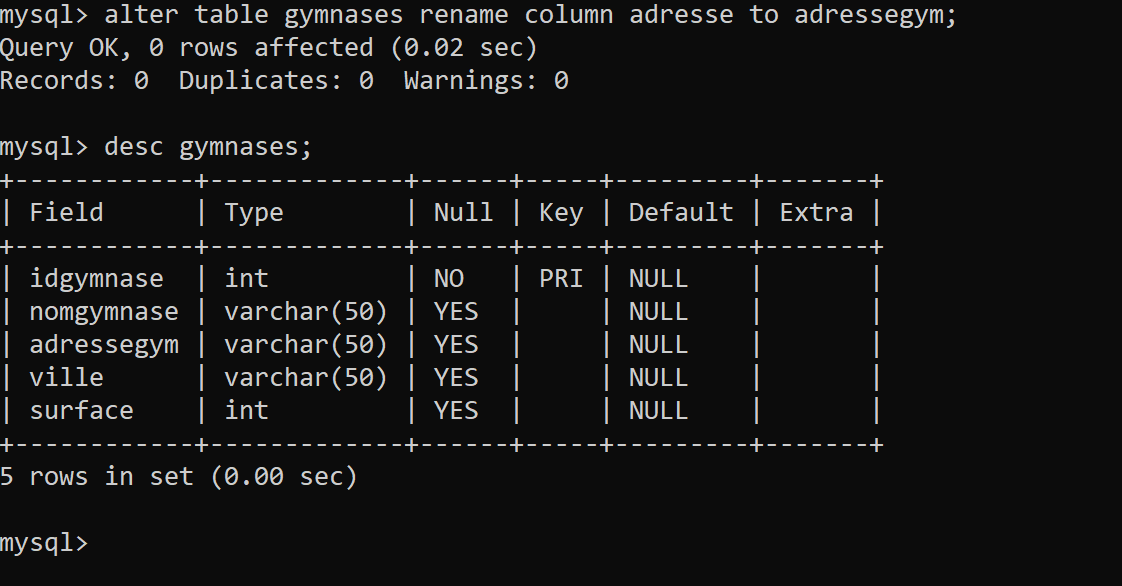
\includegraphics[height=0.36\textheight]{Parties/Partie1/rename.PNG}
\end{center}


\vspace{1cm}

\section{Ajouter La Contrainte \texttt{Check} A L'Attribut \texttt{LIBELLE} De La Table \texttt{Sports}}
\lstinputlisting{Parties/Partie1/q7.sql}




\newpage
\partie{2}
\section{Insertion}
\begin{prettyBox}{Problem}{myblue}
Il ya des erreurs d'enfrain de l'integrite de la contrainte 
\textcolor{blue}{FOREIGN KEY}
\end{prettyBox}

\vspace{0.25cm}
\textbf{\underline{Code}}
\lstinputlisting{Parties/Partie2/q8.sql}


\vspace{0.25cm}
\textbf{\underline{Output}}

\vspace{0.25cm}
\begin{center}
    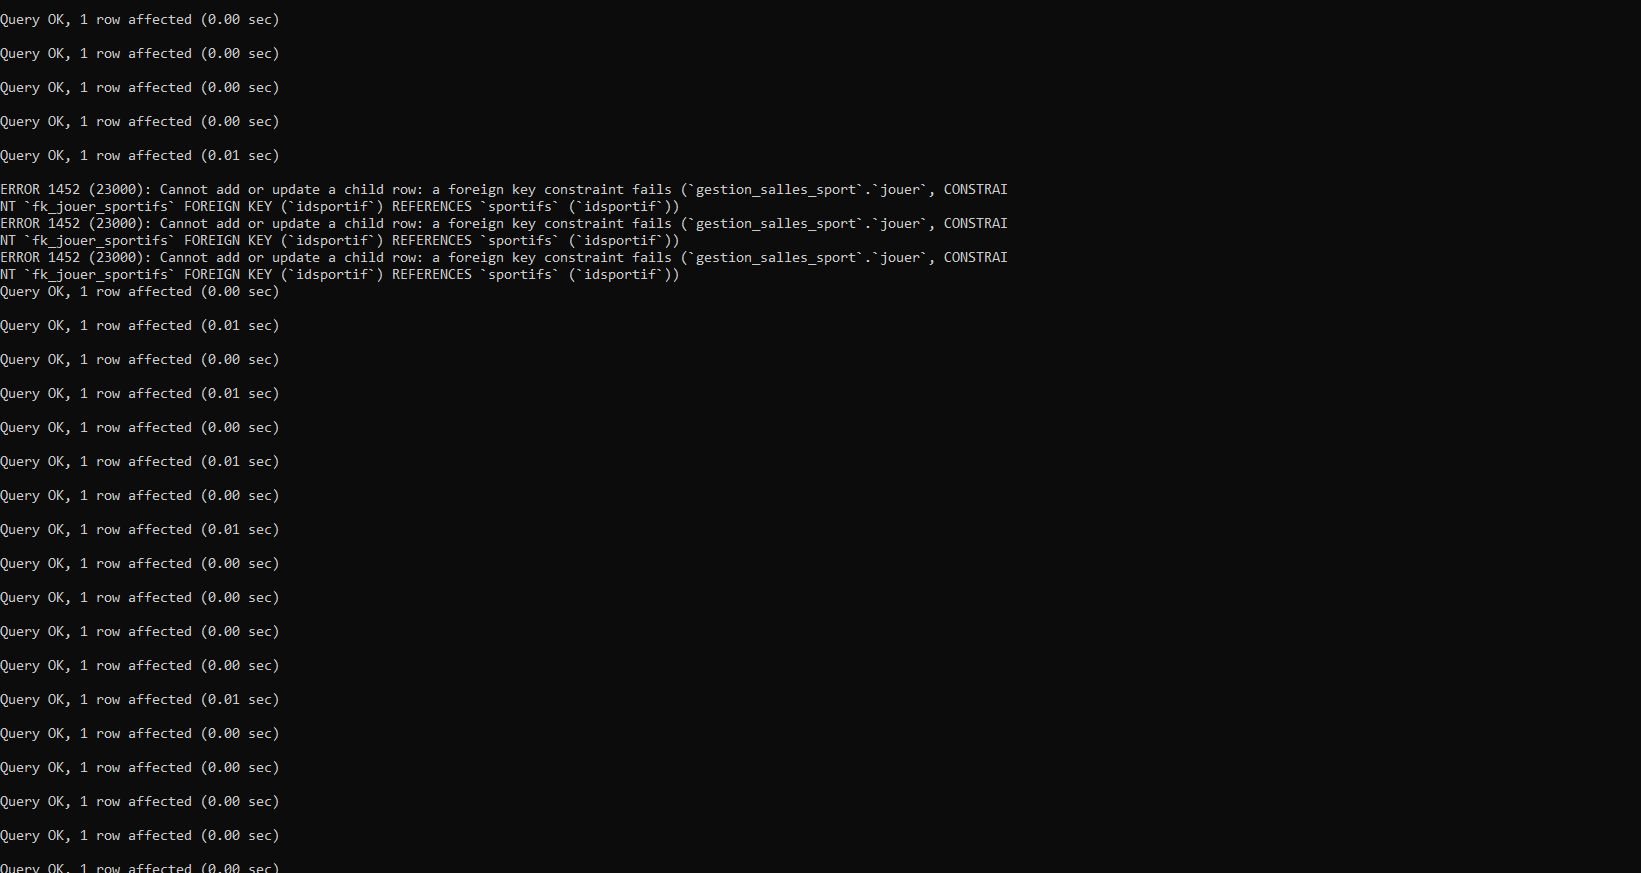
\includegraphics[width=0.8\textwidth]{Parties/Partie2/insert.PNG}
\end{center}

\newpage
\section{Changement De Conseille}
\begin{prettyBox}{Update}{myblue}
    Il est evident qu'on doit faire un \textcolor{blue}{UPDATE} sur la table \texttt{Sportifs} pour 
le sportif \texttt{LACHEMI Bouzid} pour lui change de conseille , mais d'abord
on a besoin de trouver L'\texttt{IdSportif} du nouveau Conseille \texttt{CHAADI Mourad} en 
utilisant un \textcolor{blue}{SELECT} et en stockant la valeur dans une variable qui 
va etre utilise dans l'\textcolor{blue}{UPDATE}.
\end{prettyBox}
\vspace{0.25cm}

\textbf{\underline{Code}}
\lstinputlisting{Parties/Partie2/q9.sql}

\vspace{0.25cm}
\textbf{\underline{Output}}

\vspace{0.25cm}
\begin{center}
    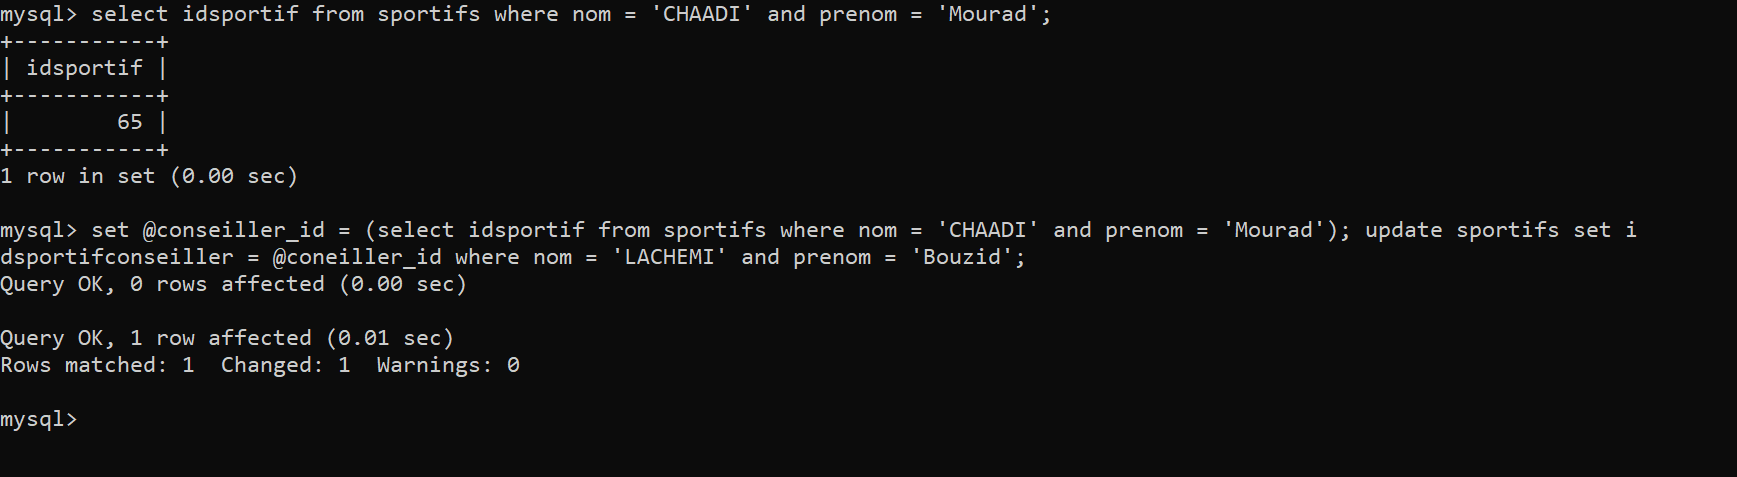
\includegraphics[height=0.25\textheight]{Parties/Partie2/update.PNG}
\end{center}

\newpage
\section{Ajout Des Deux Sport 'Natation' Et 'Golf'}
\begin{prettyBox}{Ajout}{myblue}
On ne peut pas directement inserer les sports 'Natation' et 'Golf' car 
ils ne respectent pas la contrainte \texttt{chk\_sports\_libelle} , de plus
dans \textbf{MySQL} on ne peut pas temporairment desactiver une contrainte 
avec \textcolor{blue}{DISABLE} , donc on doit supprimer la contrainte inserer et la creer a nouveau
avec un check qui accepte 'Natation' et 'Golf'.
\end{prettyBox}

\vspace{0.5cm}
\textbf{\underline{Code}}
\lstinputlisting{Parties/Partie2/q10.sql}

\vspace{1cm}
\section{Supression Des Gymnases}
\begin{prettyBox}{Problem}{myblue}
Si on essaye de supprimer n'importe quelle ligne de la table \texttt{Gymnases} , 
on aura une erreur de contrainte de la cle etrangere puisqu'elle est referance dans
la table \texttt{Seances} , si on voulais regle le problem il foudrait modifier la contrainte
\textcolor{blue}{FOREIGN KEY} en lui ajouttant \textcolor{blue}{DELETE ON CASCADE}
\end{prettyBox}

\vspace{0.5cm}
\textbf{\underline{Code}}
\lstinputlisting{Parties/Partie2/q11.sql}

\vspace{0.5cm}
\textbf{\underline{Output}}
\vspace{0.25cm}
\begin{center}
    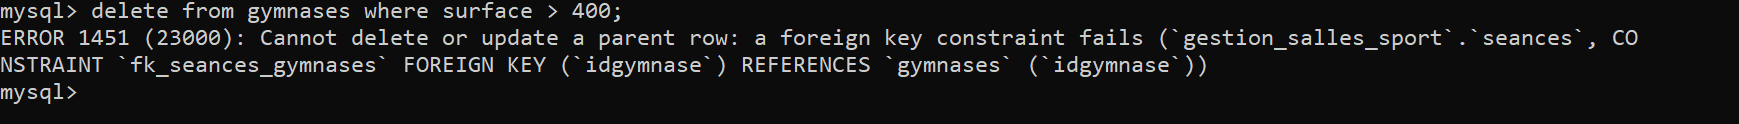
\includegraphics[width=\textwidth]{Parties/Partie2/delete.PNG}
\end{center}




\newpage
\partie{3}
\section{Sportifs Qui Ont Un Age Entre 20 Et 30}

\vspace{0.25cm}
\textbf{\underline{Code}}
\lstinputlisting{Parties/Partie3/q12.sql}


\vspace{0.25cm}
\textbf{\underline{Output}}

\vspace{0.25cm}
\begin{center}
    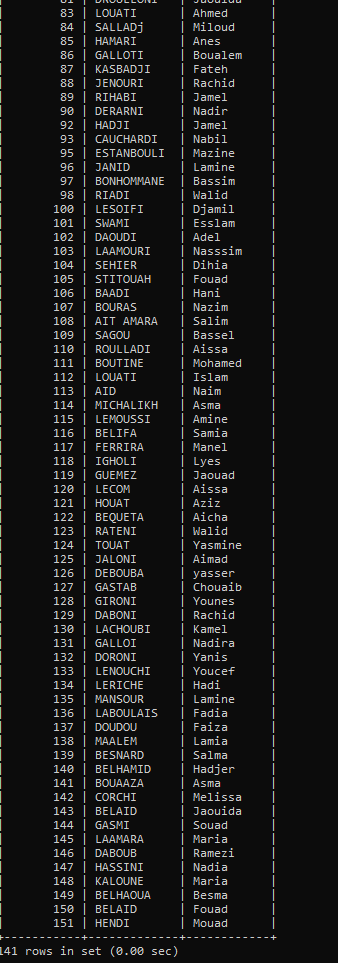
\includegraphics[height=0.6\textheight]{Parties/Partie3/sportifs.PNG}
\end{center}

\newpage

\section{Les Conseillers}
\vspace{0.25cm}
\textbf{\underline{Code}}
\lstinputlisting{Parties/Partie3/q13.sql}


\vspace{0.25cm}
\textbf{\underline{Output}}

\vspace{0.25cm}
\begin{center}
    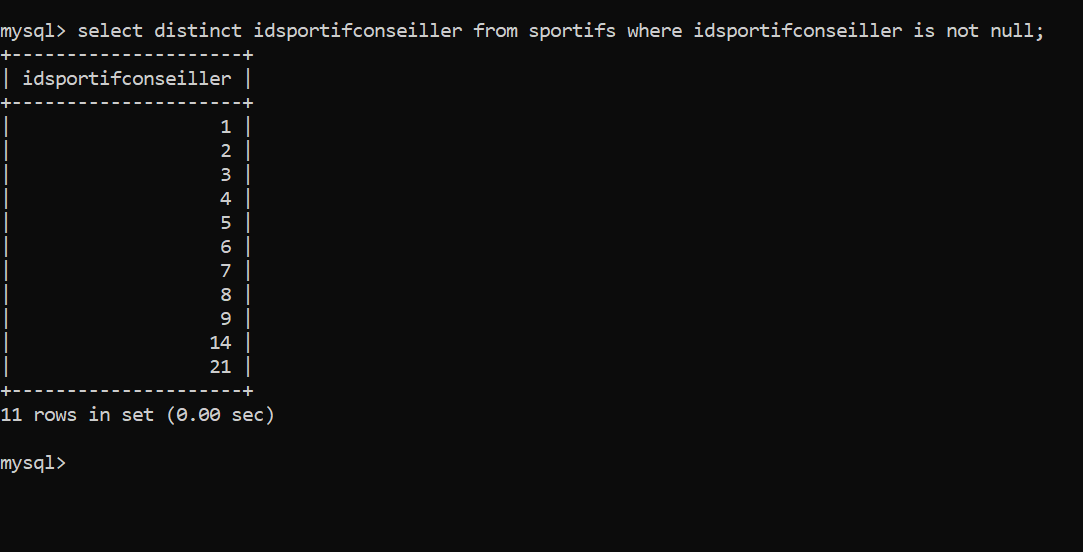
\includegraphics[width=0.8\textwidth]{Parties/Partie3/conseiller.PNG}
\end{center}

\vspace{0.25cm}
\begin{prettyBox}{Remarque}{red}
On a utilise \textcolor{blue}{DISTINCT} parceque l'attribut \texttt{IdSportifConseiller} est une
cle strangere donc elle peut etre repete sure plusieur lignes , et on a verifie si l'id ete \textcolor{blue}{NULL} ,
pour filtrer les valeur \textcolor{blue}{NULL} (sportifs sans conseiller)
\end{prettyBox}

\newpage
\section{Entraineur De Hand-Ball Ou Basket-Ball}

\begin{prettyBox}{Explication}{myblue}
\textbf{\underline{Soit Hand-Ball, Soit Basket-Ball, Ou Les Deux}} \\[0.15cm]
On a un \textcolor{blue}{SELECT} imbriqué où la subquery nous donne les \texttt{IdSportifEntraineur}
qui n'ont pas entraîné au moins une foit 'Hand-Ball' ou 'Basket-Ball',  
en effectuant une jointure entre les tables \texttt{Entrainer} et \texttt{Sports} avec
un \textcolor{blue}{NOT IN} pour récupérer les \texttt{LIBELLE}.  
L'outer query sélectionne les \texttt{IdSportifEntraineur} qui ne font pas partie de cet ensemble,  
ce qui revient à obtenir les entraîneurs qui pratiquent exclusivement le Hand-Ball ,le Basket-Ball, ou les deux.
\vspace{0.25cm}

\textbf{\underline{Soit Hand-Ball, Soit Basket-Ball Uniquement}} \\[0.15cm]
Même logique, sauf que cette fois, on utilise deux requêtes avec \textcolor{blue}{UNION} :  
la première récupère les IDs des entraîneurs qui ne pratiquent aucun sport autre que le Hand-Ball,  
et la seconde ceux qui ne pratiquent aucun sport autre que le Basket-Ball.  
La différence réside dans l'ensemble utilisé dans le \textcolor{blue}{NOT IN}.
\end{prettyBox}
\vspace{0.5cm}
\textbf{\underline{Code}}
\lstinputlisting{Parties/Partie3/q14.sql}

\vspace{0.5cm}
\textbf{\underline{Output}}

\vspace{0.25cm}
\begin{center}
    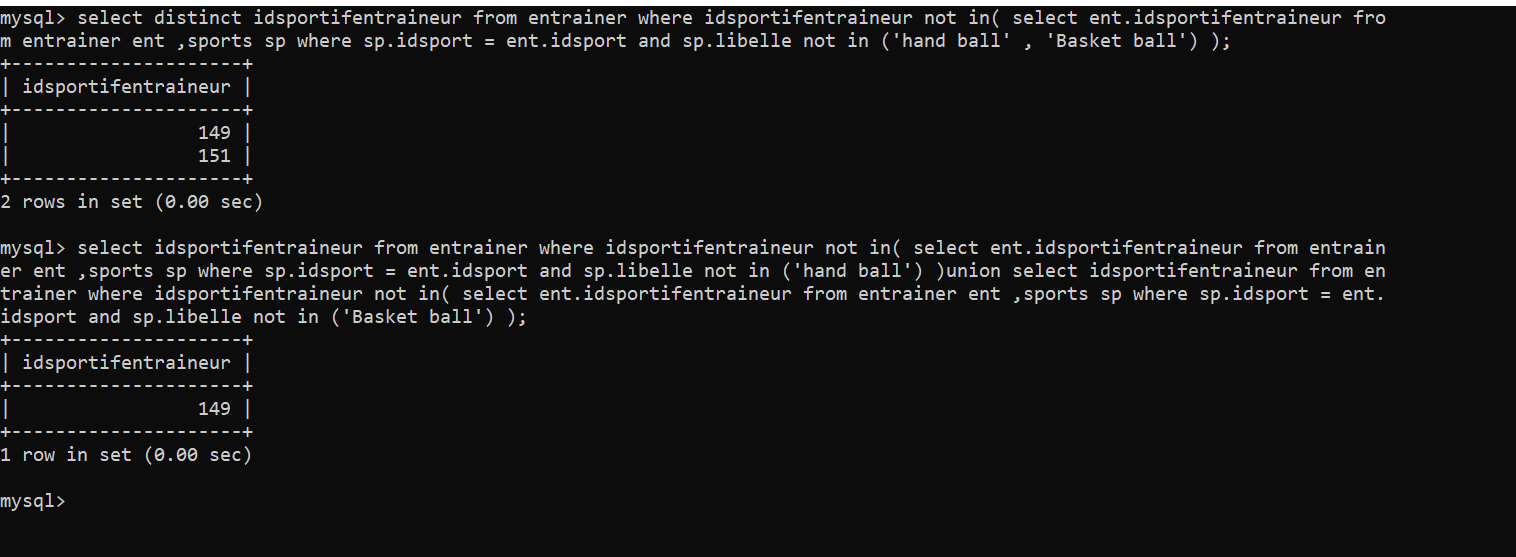
\includegraphics[width=0.8\textwidth]{Parties/Partie3/ent.PNG}
\end{center}

\newpage

\section{Sportifs Les Plus jeunes}

\textbf{\underline{Code}}
\lstinputlisting{Parties/Partie3/q15.sql}

\vspace{0.5cm}
\textbf{\underline{Output}}

\vspace{0.25cm}
\begin{center}
    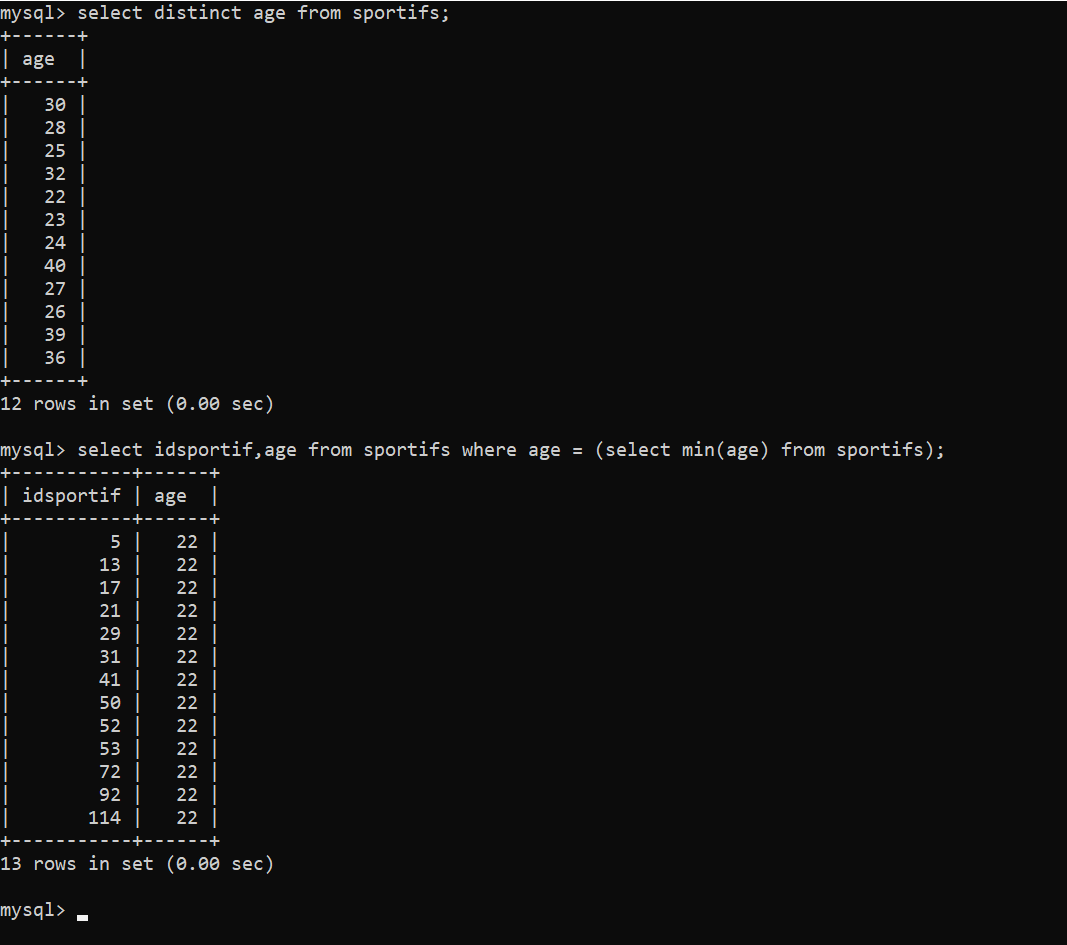
\includegraphics[width=0.8\textwidth]{Parties/Partie3/age.PNG}
\end{center}

\newpage

\section{Superficie Moyennes Des Gymnases Par Ville}

\textbf{\underline{Code}}
\lstinputlisting{Parties/Partie3/q16.sql}

\vspace{0.5cm}
\textbf{\underline{Output}}

\vspace{0.25cm}
\begin{center}
    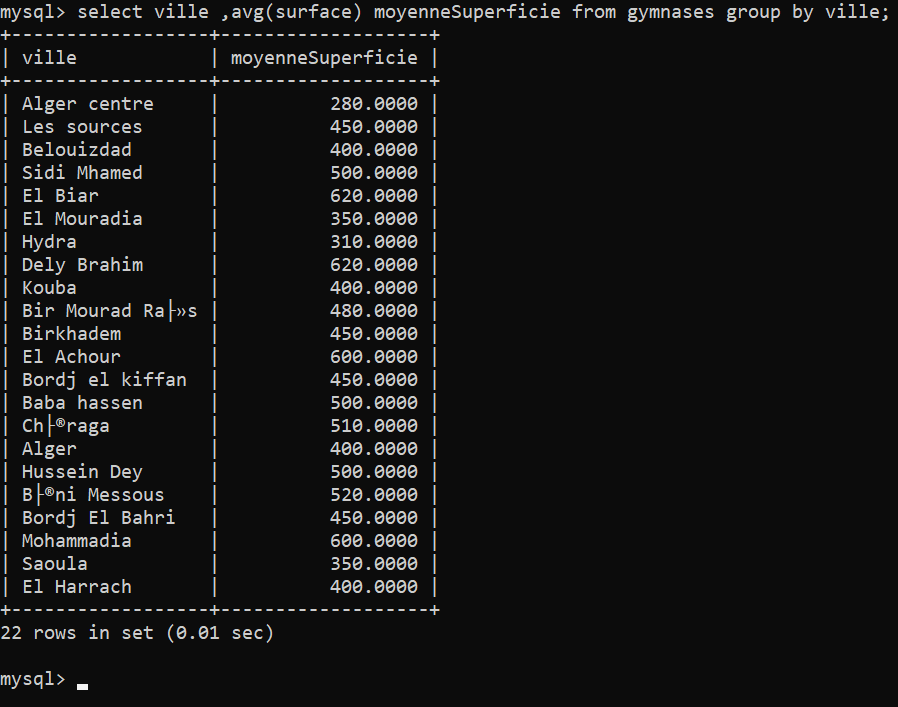
\includegraphics[width=0.8\textwidth]{Parties/Partie3/avg.PNG}
\end{center}

\newpage

\section{Ville Avec Le Plus Grand Nombre De Gymnases}

\textbf{\underline{Code}}
\lstinputlisting{Parties/Partie3/q17.sql}

\vspace{0.5cm}
\textbf{\underline{Output}}

\vspace{0.25cm}
\begin{center}
    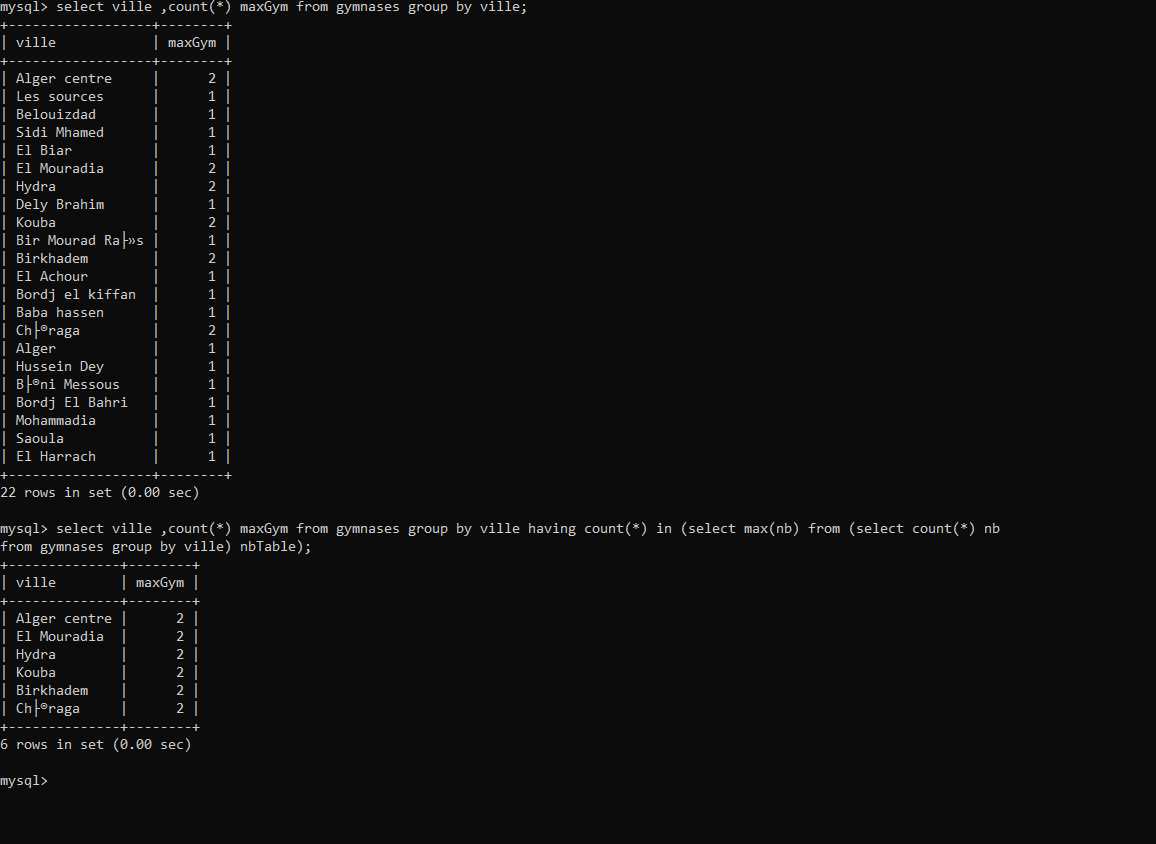
\includegraphics[width=0.8\textwidth]{Parties/Partie3/nbgym.PNG}
\end{center}

\vspace{0.5cm}

\begin{prettyBox}{Note}{red}
On ne peut pas utiliser \textcolor{blue}{COUNT(*)} comme paramètre dans \textcolor{blue}{MAX},  
donc on est obligé d'utiliser une subquery qui génère la table qui contient la colonne des  
nombres de gymnases pour chaque ville.
\end{prettyBox}


\end{document}
